\newcolumntype{M}[1]{>{\raggedleft}m{#1}}

\chapter{Tests}

Afin de déterminer les limites de notre application, nous avons effectué une série de tests pour découvrir les comportements anormaux et se rassurer sur la stabilité de notre projet.\newline
Tous les tests ont été effectués en appelant les fonctions que le frontend utilise. Ce qui permettait de mesurer plus précisément les actions du frontend ou de l'API. Pour la majorité des tests, accéder à l'interface graphique n'était pas utile.

Les mesure de temps pour les tests sur l'API ont été obtenues par le système de "tests" de Django.
Les mesure de temps pour les tests sur l'interface ont été obtenues lors du chargement d'une "view" de Django.

\section{Tests unitaire}
Dans chaque micro service que l'on a mis en place, nous avons des tests unitaires. Pour leur réalisation, nous avons essayer d'obtenir le plus de couverture de code possible.
Les tests réalisés se placent dans le cadre de tests end-to-end.


Nous avons donc les couverture suivante pour le frontend :
\begin{figure}[H]
    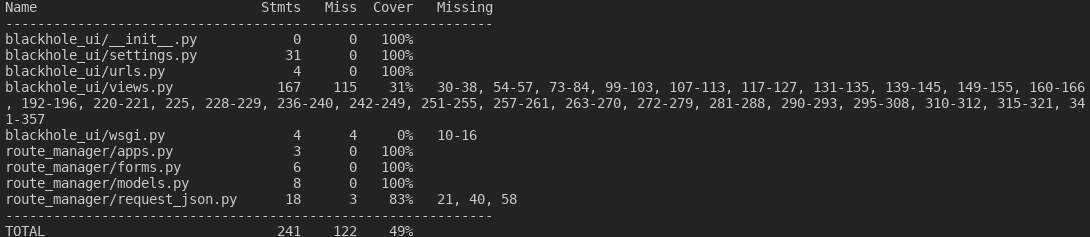
\includegraphics[width=\textwidth]{frontend_coverage.png}
    \caption{Couverture du frontend}
    \label{fig:front}
\end{figure}

Et sur le backend:
\begin{figure}[H]
    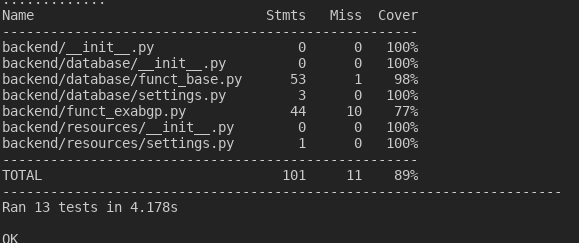
\includegraphics[width=\textwidth]{backend_coverage.png}
    \caption{Couverture du backend}
    \label{fig:back}
\end{figure}

Comme on peut le voir sur le frontend, il nous manque des test sur le fichier \verb+view.py+
Mis à part cela, nous sommes assez satisfait de la couverture que l'on obtient.

\section{Test d'intégration}
Afin de garantir que notre code soit toujours fonctionnel, nous avons mis en place de l'intégration continue grâce à Travis CI. Il nous permet de vérifier que le fichier de requirements.txt soit toujours à jour et que les tests du backend soit toujours opérationnels. Ensuite, nous utilisons sonar cloud afin d'avoir une qualité de code élevée.

Cette intégration continue est une vrai plu value que nous avons eu envie de mettre en place pour expérimenter des techniques de Génie Logiciel même si on est pas dans cette section.


%\section{Scénario }
% A renommer

%\section{Tests d'acceptation}
%Dans un premier temps, l'utilisateur met en place son environnement virtuel. Pour cela, les commandes sont disponibles dans le README.md.
% a voir si on détaille toutes les commandes pour la générer, mettre une configuration/topologie, détailler topo
%Une fois cela effectué, l'utilisateur peut accéder à l'interface de connexion de l'application.

% préciser comment il y accède
%'utilisateur peut s'authentifier avec ses identifiants, si un compte à été créée.

%Cependant, s'il oublie son mot de passe, il aura la possibilité de le récupérer grâce au lien \textit{Mot de passe oublié ?} situé en dessous de ces deux champs. Actuellement il n'est pas possible de récupérer un mot de passe perdu à l'aide d'un mail. Nous n'avons pas déployé de service de mail pour cette tâche.
%Recréer un compte est plus rapide et ne provoque aucune différence.
%Imaginons, qu'il l'a effectivement oublié. Il clique donc sur \textit{Mot de passe oublié ?} et une nouvelle fenêtre s'ouvre lui demandant d'entrer son adresse e-mail. Une fois cela fait, il clique sur \textit{Envoyer}. Si tout se passe bien, il devrait recevoir un e-mail avec son mot de passe.

% pas safe à voir
%Une fois les deux champs remplis, l'utilisateur clique sur \textit{Log In}. L'utilisateur sera redirigé vers l'interface de l'application, lui permettant d'exécuter différentes actions.

%La premier chose que l'utilisateur voit est le voyant, attestant de la bonne ou mauvaise fonctionnalité. Le voyant étant vert, l'application fonctionne.

% détailler si le voyant est rouge.
%Ensuite, il peut attester de son identité et voit tous ses réseaux.

%Il a précédemment remarqué qu'un trafic trop important se dirigeait vers l'un de ses serveurs.

%Après étude, il en ressort l'adresse IP attaquante et l'adresse IP cible. A ce stade, il y a trois choix possibles. Soit l'utilisateur décide de router par source, par destination ou par communautés. Nous allons étudier ces trois cas.

%Il va donc neutraliser l'attaquant en changeant le routage vers la cible. Il veut maintenant ajouter une route pour rediriger l'attaque vers un trou noir. Dans le champs \textit{IP ou réseau}, il renseigne l'adresse attaquante. Dans \textit{Prochain saut}, il renseigne le prochain saut vers un trou noir, sachant qu'il a le droit à une liste. Ensuite, il peut sélectionner la ou les communautés à laquelle il veut appliquer cette modification. Une fois cela fait, il peut cliquer sur \textit{Valider}.

%A ce moment, une requête HTTP est envoyé de l'interface utilisateur vers l'API. Celle-ci envoie une requête à ExaBGP. ExaBGP va donc diffuser la nouvelle route sur le réseau. Une fois cela effectué, ExaBGP envoie une réponse à l'API. Deux cas sont donc possibles : la diffusion a réussi ou elle a échoué.

%Prenons le cas de la réussite. L'API va donc mettre à jour la base de données. Cela fait, l'utilisateur verra apparaître le changement sur son interface.

%Si la diffusion de la route échoue, l'API ne modifiera pas la base de données. Elle enverra une requête à l'interface utilisateur qui affichera un message d'erreur.

%Quelques temps plus tard, le trafic semble s'être réduit. L'utilisateur a donc deux choix possibles : Supprimer la route qu'il a précédemment créé ou tout simplement la désactiver.

%Commençons par cette seconde option. L'utilisateur, ne sait pas si le problème reviendra plus tard. Il décide donc de désactiver la route précédemment créée. Les informations seront toujours contenues dans la base de données. Cela lui évitera de la saisir de nouveau. Il va donc sélectionner la route et cliquer pour la désactiver. Une requête est donc envoyée à l'API qui va elle-même en envoyer une a ExaBGP pour diffuser le nouveau message sur les routeurs et la route n'existera donc plus sur la table de routage de ceux-ci. Après avoir reçu la réponse d'ExaBGP, l'API va mettre à jour la base de données de la même manière qu'expliquée précédemment. La route sera toujours présente dans la base de données.

%Prenons maintenant la deuxième option. L'utilisateur sélectionne simplement la route précédemment créée et clique pour la supprimer. Une requête est envoyée à l'API, et de la même manière que la désactivation une diffusion est envoyée aux routeurs et la routes n'existe donc plus sur la table de routage de ceux-ci, ni sur la base de données. \\ \indent
%Il y a de nouveau une attaque venant de la même adresse IP. Si l'utilisateur a supprimé la route, il est obligé de la créer de nouveau. S'il l'a désactivée, il n'aura qu'à la sélectionner et l'activer.

%Dans ce deuxième cas, il va générer un routage par destination. Tout le trafic se dirigeant vers son serveur sera redirigé vers un trou noir.

%détailler par dest


%détailler par communautés
%Dans le cas ou l'utilisateur souhaite faire un routage par communauté, il pourra diffuser une demande de routage qui s'appliquera à tout les membres de la communauté sans s'appliquer aux autres.

%L'utilisateur souhaite maintenant quitter sa session. Il clique sur son identité. Un bouton \textit{Déconnexion} apparaît. Il clique dessus. L'utilisateur est redirigé sur l'interface de connexion. Il ne peut plus rien faire sauf entrer ses identifiants de nouveau ou faire une demande suite à l'oubli de son mot de passe.

\newpage

\section{Tests de performances}

Le premier test visait à déterminer la vitesse d'action de l'API.\newline
On demande à l'API de créer et supprimer plusieurs quantité différentes de routes, le plus rapidement possible.\newline


%Table création
\begin{footnotesize}
\small
\centerline{}
\begin{tabular}{ | M{2cm} || c | c | c | c | c |c | c | c | c | }
 \hline
\textbf{Routes} & 1 & 2 & 4 & 8 & 16 & 32 & 64 & 128 & 256\\
\hline
\textbf{Temps création total\\(secondes)} & 0,538 & 0,538 & 1,424 & 2,574 & 5,153 & 10,118 & 20,861  & 40,488 & 79,755\\
\hline
\textbf{Temps création unité\\(secondes)} & 0,538 & 0,269 & 0,356 & 0,322 & 0,322 & 0,316 & 0,326 &	0,316 &	0,312\\
\hline

%Graph création
\end{tabular}
\end{footnotesize}
\begin{figure}[H]
    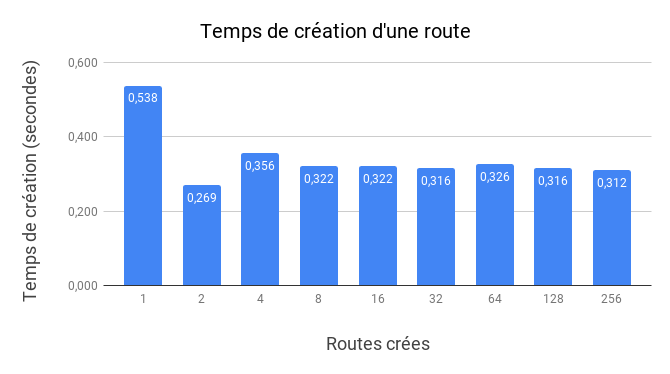
\includegraphics[width=\textwidth]{creation_route_time.png}
    %\caption{Diagramme d'utilisation de l'application}
    %\label{fig:use_cases}
\end{figure}
\newpage
%Table suppression
\begin{footnotesize}
\small
\centerline{}
\begin{tabular}{ | M{3cm} || c | c | c | c | c |c | c | c | c | }
 \hline
\textbf{Routes} & 1 & 2 & 4 & 8 & 16 & 32 & 64 & 128 & 256\\
 \hline
\textbf{Temps suppression total(secondes)} & 0,811 & 1,118 & 1,708 & 2,92 & 5,638 & 10,357 & 20,272 & 39,964 & 79,852\\
 \hline
\textbf{Temps suppression unité(secondes)} & 0,811 & 0,559 & 0,427 & 0,365 & 0,352 & 0,324 & 0,317 & 0,312 & 0,312\\
 \hline
 \end{tabular}
\end{footnotesize}

%Graph suppression
\begin{figure}[H]
    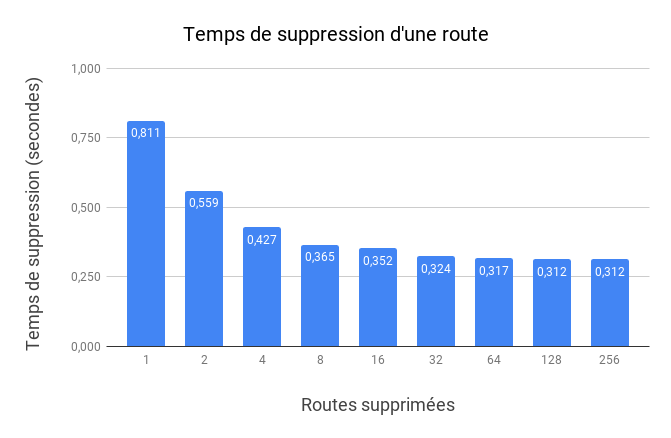
\includegraphics[width=\textwidth]{deletion_route_time.png}
    %\caption{Diagramme d'utilisation de l'application}
    %\label{fig:use_cases}
\end{figure}


Ce premier test nous permet de découvrir qu'il faut, en moyenne, \textbf{320 ms pour ajouter ou supprimer une route} en demandant directement à l'API.
On peut expliquer l'écart entre la valeur moyenne et les premières valeurs par l'environnement de test Django qui met du temps à se déployer (200-500 ms). Un délai qui deviens négligeable plus l'on manipule de routes.



\newpage
Le second test de performance visait à déterminer le comportement de l'application lors d'une utilisation "normale". \newline
On demande à l'API d'ajouter progressivement des routes et ensuite on mesure le temps de chargement de l'interface (dashboard).\newline

\begin{figure}[H]

    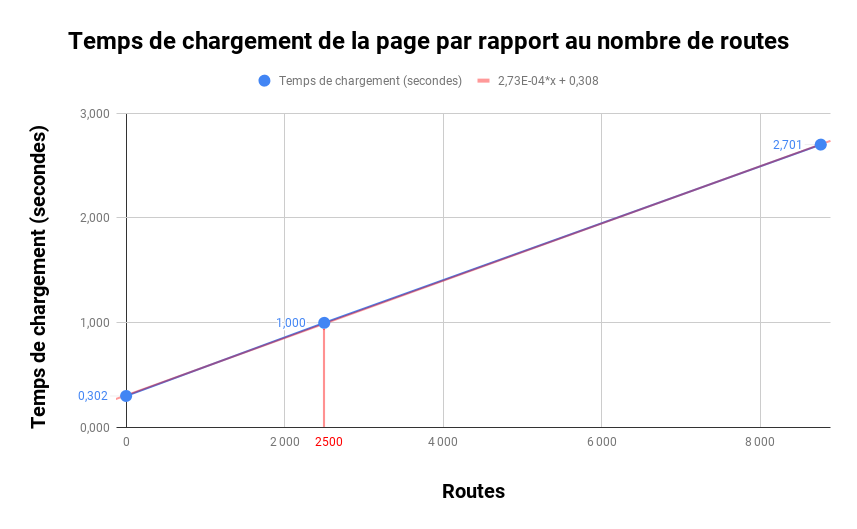
\includegraphics[width=\textwidth]{small_scale.png}

\end{figure}

Ce second test nous permet de découvrir que, en moyenne, \textbf{l'interface prendra une seconde pour charger 2500 routes}.

\newpage % je voulais pas mettre de newpage mais j'ai pas le choix, les images prennent trop de place
Le troisième test de performance visait à déterminer le comportement de l'application et l'API lors d'une utilisation "anormale".\newline
En utilisant 20 terminaux qui vont agir en parallèle pendant une heure, on demande à l'API d'ajouter le plus rapidement possible des routes.Pendant cett période on mesure régulièrement le temps de chargement de l'interface (dashboard).\newline



\begin{figure}[H]
    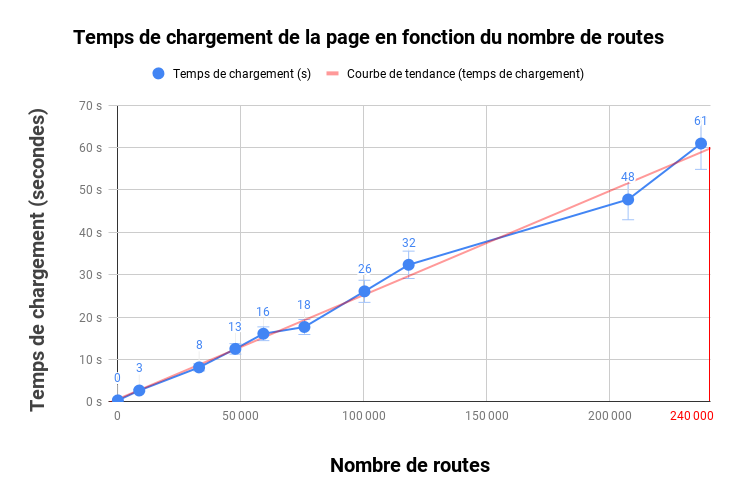
\includegraphics[width=\textwidth]{big_scale.png}
\end{figure}

Ce troisième test nous permet de découvrir que, en moyenne, \textbf{l'interface prendra une minute pour charger 240.000 routes} et que \textbf{l'API peut supporter 560 appels par seconde}.

\newpage




\section{Tests des fonctionnalités}

Ces tests utilisent l'environnement de test de Django et ont pour but de vérifier les fonctionnalités principales de l'application.
Une base de donnée temporaire est crée à chaque série de test.\\

\underline{Authentification} :
\begin{itemize}
\item Un utilisateur dans la base de données peut se connecter
\item un utilisateur qui n'est pas dans la base de données ne peut pas se connecter
\item un utilisateur authentifié peut accéder à du contenu restreint
\item un utilisateur anonyme ne peut pas accéder à du contenu restreint\newline
\end{itemize}


\underline{API} :
\begin{itemize}
\item L'API doit être atteignable
\item une route créée puis supprimée doit correspondre aux paramètres spécifiés\newline
\end{itemize}

\underline{Frontend} :
\begin{itemize}
\item le formulaire doit permettre la création de routes correct
\item le formulaire doit bloquer la création de routes incorrectes
\end{itemize}

